\chapter{Исследовательская часть}

\section{Прмиер работы}
Демонстрация работы программы приведена на рисунке 4.1

\begin{figure}[h]
	\centering
	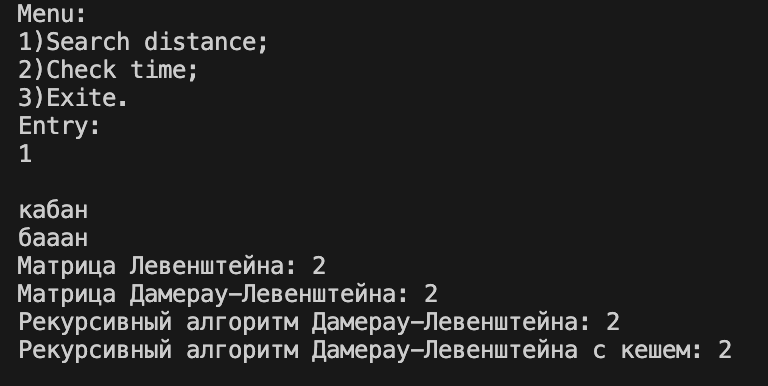
\includegraphics[height=0.2\textheight]{img/example.jpg}
	\caption{Демонстрация работы программы при поиске расстояний Левенштейна и Дамерау-Левенштейна}
	\label{img:demonstration}
\end{figure}

\section{Технические характеристики}

Технические характеристики устройства, на котором выполнялись замеры по времени, представлены далее.

\begin{itemize}
	\item Процессор:2 GHz 4‑ядерный процессор Intel Core i5.
	\item Оперативная память: 16 ГБайт.
	\item Операционная система: macOS Venura 13.5.2. 
\end{itemize}

\clearpage

\section{Время выполнения алгоритмов}

Результаты эксперимента замеров по времени приведены в таблице 4.2. В данной
таблице присутствуют поля с «-». Это обусловлено тем, что для 
рекурсивной реализации алгоритма достаточно приведенных замеров для 
построения графика. При длине строки большей 10 замер времени для рекурсивного
алгоритма будет достаточно долгим.
Замеры проводились на одинаковых длин строк от 1 до 1000 с различным шагом.

\begin{figure}[h]
	\centering
	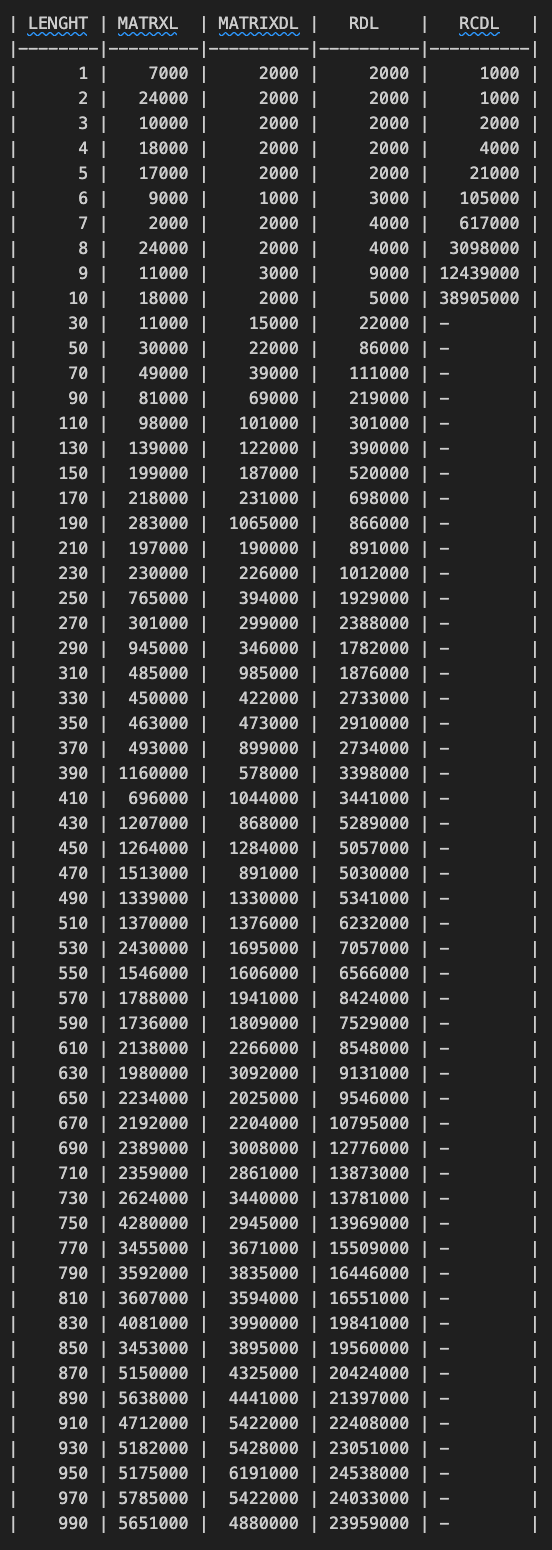
\includegraphics[width=0.37\textwidth]{img/resultTime.jpg}
	\caption{Демонстрация работы программы при поиске расстояний Левенштейна и Дамерау-Левенштейна}
	\label{img:demonstration}
\end{figure}

\begin{figure}[h]
	\centering
	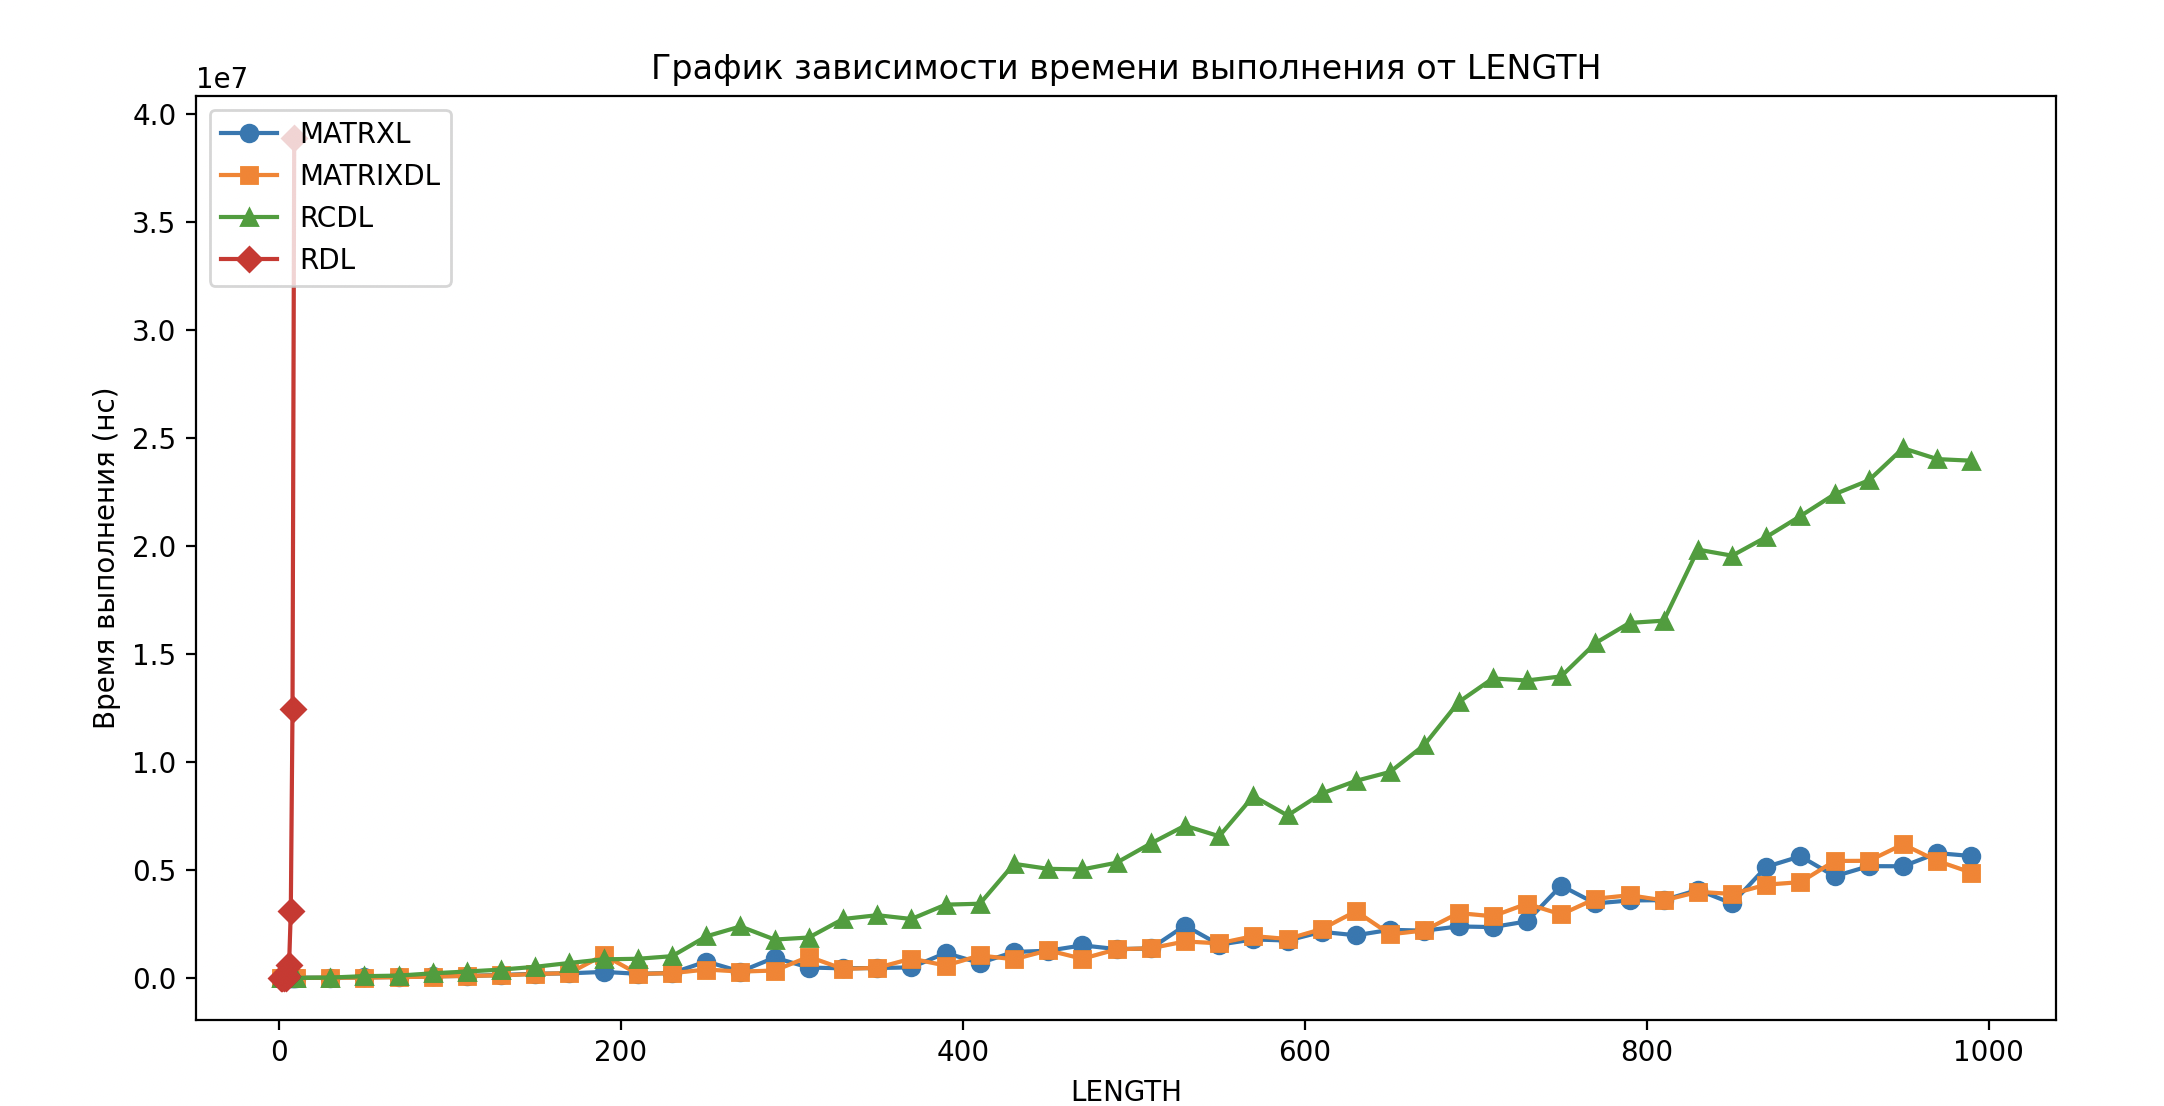
\includegraphics[width=1\textwidth]{img/graphic_2.jpg}
	\caption{График работы программы при поиске расстояний Левенштейна и Дамерау-Левенштейна}
	\label{img:demonstration}
\end{figure}

При длинах строк менее 200 символов разница по времени между 
итеративными реализациями и рекурсивной с кешем незначительна, 
однако при увеличении 
длины строки алгоритм рекурсивного поиска расстояния Дамерау-Левенштейна с кешем 
оказывается медленнее вплоть до 4 раз(при длинах строк равных 990). 

Если рассматривать итерационные алгоритмы, то алгоритм Левенштейна работает немного быстрее,
чем алгоритм Дамерау-Левенштейна, так как во втором есть дополнительная проверка.

Алгоритмы нахождения расстояния Левенштейна и Дамерау — Левенштейна не отличаются друг от друга с точки зрения использования памяти.

Максимальная глубина стека вызовов при рекурсивной реализации равна сумме длин входящих строк. Поэтому, максимальный расход памяти равен: 

\clearpage

\section{Использование памяти}

\begin{equation}
(\mathcal{S}(STR_1) + \mathcal{S}(STR_2)) \cdot (2 \cdot \mathcal{S}\mathrm{(string)} + 3 \cdot \mathcal{S}\mathrm{(integer)}),
\end{equation}

\noindent где $\mathcal{S}$ — оператор вычисления размера, $STR_1$, $STR_2$ — строки, $\mathrm{string}$ — строковый тип, 

\noindent $\mathrm{integer}$ — целочисленный тип.

Использование памяти при итеративной реализации теоретически равно:
\begin{equation}
(\mathcal{S}(STR_1) + 1) \cdot (\mathcal{S}(STR_2) + 1) \cdot \mathcal{S}\mathrm{(integer)} + 5\cdot \mathcal{S}\mathrm{(integer)} + 2 \cdot \mathcal{S}\mathrm{(string)}.
\end{equation}

\section{Вывод}

В данном разделе было произведено сравнение количества затраченного времени 
и памяти алгоритмов поиска расстояний Левенштейна и Дамерау-Левенштейна. 
Наименее затратным по времени оказался итеративный алгоритм нахождения расстояния 
Левенштейна.

Приведенные характеристики показывают, что рекурсивная реализация алгоритма 
во много раз проигрывает по времени. В связи с этим, рекурсивные алгоритмы следует 
использовать лишь для малых размерностей строк (<= 10 символов).

Так как во время печати очень часто возникают ошибки связанные с 
транспозицией букв, алгоритм поиска расстояния Дамерау-Левенштейна 
является наиболее предпочтительным, не смотря на то, что он незначительно 
проигрывает по времени и памяти алгоритму Левенштейна.

